\chapter{Технологический раздел}

\section{Средства разработки}

Для реализации поддерживающего спроектированный протокол ПО был выбран язык С.
В качестве средства сборки используется средство сборки CMake \cite{cmake}.

Для работы с медиа данными используется библиотека с открытым исходным кодом \texttt{ffmpeg} \cite{ffmpeg}.

Шифрование сообщений осуществляется с использованием библиотеки \texttt{OpenSSL}.

Для автотестов используется фреймворк \texttt{GoogleTest} \cite{gtest}.

\section{Листинги процедуры приглашения}

\includelisting
  {invite-clnt}
  {Процедура приглашения со стороны приглашающего}

\includelisting
  {invite-srv}
  {Процедура приглашения со стороны приглашаемого}

\includelisting
  {invite-worker}
  {Воркер, обрабатывающий входящие приглашения в конференции}

\includelisting
  {invite}
  {Процедура приглашения участника в конференцию}

\section{Сборка и запуск}

Сборка основного проекта осуществляется с использованием утилиты cmake:

\begin{verbatim}
  mkdir build
  cd build
  cmake ..
  make цель
\end{verbatim}
где \textit{<<цель>>} может быть \texttt{selecon\_cli} для сборки консольной утилиты, либо \texttt{unittests} для сборки тестов.

Консольная утилита имеет следующие параметры запуска:

\begin{verbatim}
$ ./selecon_cli --help
./selecon_cli [OPTIONS]

  example demo application for selecon protocol

OPTIONS:
  -h|--help              show this message
  -l|--listen-on address current participant address (default 0.0.0.0:11235)
  -u|--user username     set user name
  --version              print version and exit
  --stub filename        stream given media file in a loop

DESCRIPTION:
  Address can be IPv4/IPv6 (eg: 192.168.100.1:11235) or socket file path
  in format file://<os-path-to-socket>.
\end{verbatim}

Список команд, поддерживаемых утилитой:

\begin{verbatim}
$ ./selecon_cli
> help
list of available commands:
  dev     manage IO devices
  dump    print info about current selecon context state
  exit    end active conference and close cli tool
  help    show this message
  invite  send invitation for joining active conference to other client
  leave   exit conference without exiting cli tool
  quit    same as exit
  say     send text message to conference chat
  sleep   sleep
  stub    set stub media file for playing in conference
\end{verbatim}

В качестве видео заглушки можно использовать видео файлы в формате MP4.

\clearpage

\section{Тестирование ПО}

Ниже приведен список автотестов, разработанных для проверки реализованного протокола. 

\begin{itemize}[label=---]
  \item Подключение второго участника к конференции, второй участник отклонил приглашение.
  \item Подключение второго участника к конференции, второй участник принял приглашение.
  \item Отправка аудио данных от одного участника другому.
  \item Отправка видео данных от одного участника другому.
  \item Подключение четырех участников к конференции.
  \item Отправка аудио данных от одного участника к другим трем.
  \item Отправка видео данных от одного участника к другим трем.
\end{itemize}

\section{Трасировка пакетов}

На рисунке \ref{img:trace-conf-2} представлен сниф пакетов с использованием программы wireshark \cite{wireshark} во время инициализации конференции с двумя участниками.
На рисунке \ref{img:trace-conf-2-tls} представлен сниф того же сценария, но с использованием TLS протокола.

\begin{figure}[h!]
  \centering
  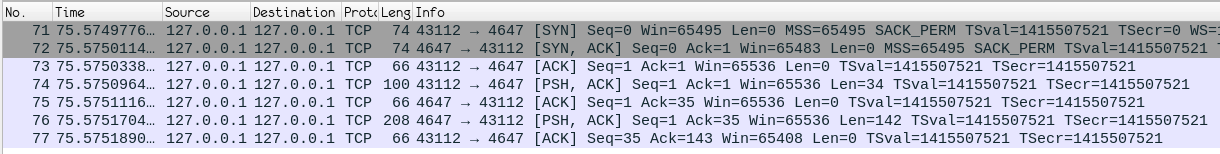
\includegraphics[width=\linewidth]{inc/img/trace-conf-2.png}
  \caption{Сниф wireshark соединения двух участников без использования TLS}
  \label{img:trace-conf-2}
\end{figure}

\begin{figure}[h!]
  \centering
  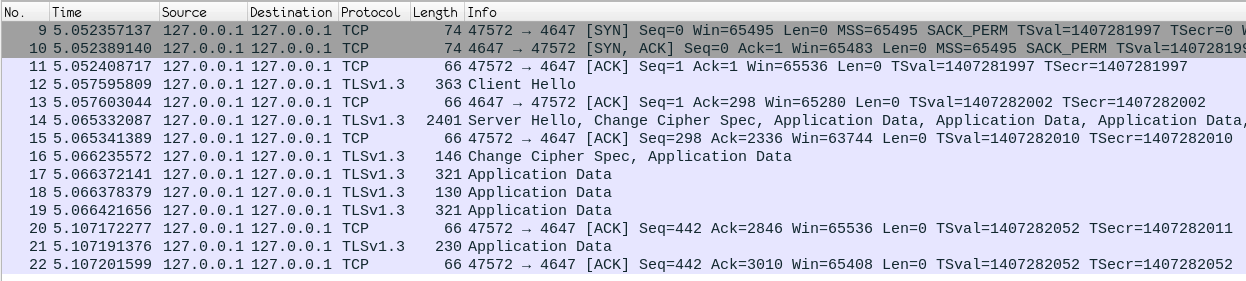
\includegraphics[width=\linewidth]{inc/img/trace-conf-2-tls.png}
  \caption{Сниф wireshark соединения двух участников с использованием TLS}
  \label{img:trace-conf-2-tls}
\end{figure}

\clearpage

На рисунках \ref{img:trace-conf-3}--\ref{img:trace-conf-3-tls} представлены снифы пакетов во время инициализации конференции с тремя участниками. По рисунку видны 3 этапа соединения: инициализация конференции двумя участниками; отправка и получение приглашения для третьего участника и информирование второго участника о новом подключившемся участнике; рукопожатие второго и третьего участников.

\begin{figure}[h!]
  \centering
  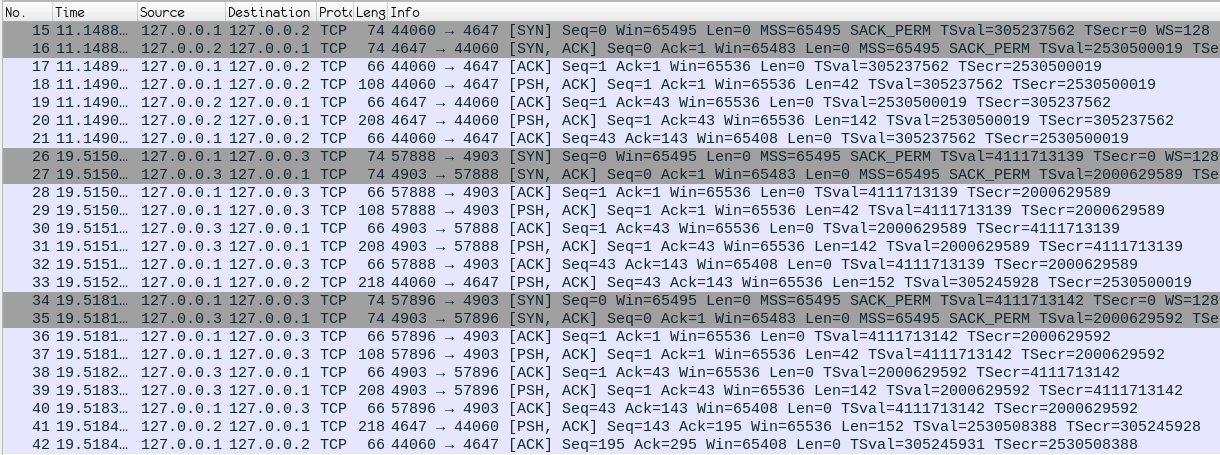
\includegraphics[width=\linewidth]{inc/img/trace-conf-3.png}
  \caption{Сниф wireshark соединения трех участников без использования TLS}
  \label{img:trace-conf-3}
\end{figure}

\begin{figure}[h!]
  \centering
  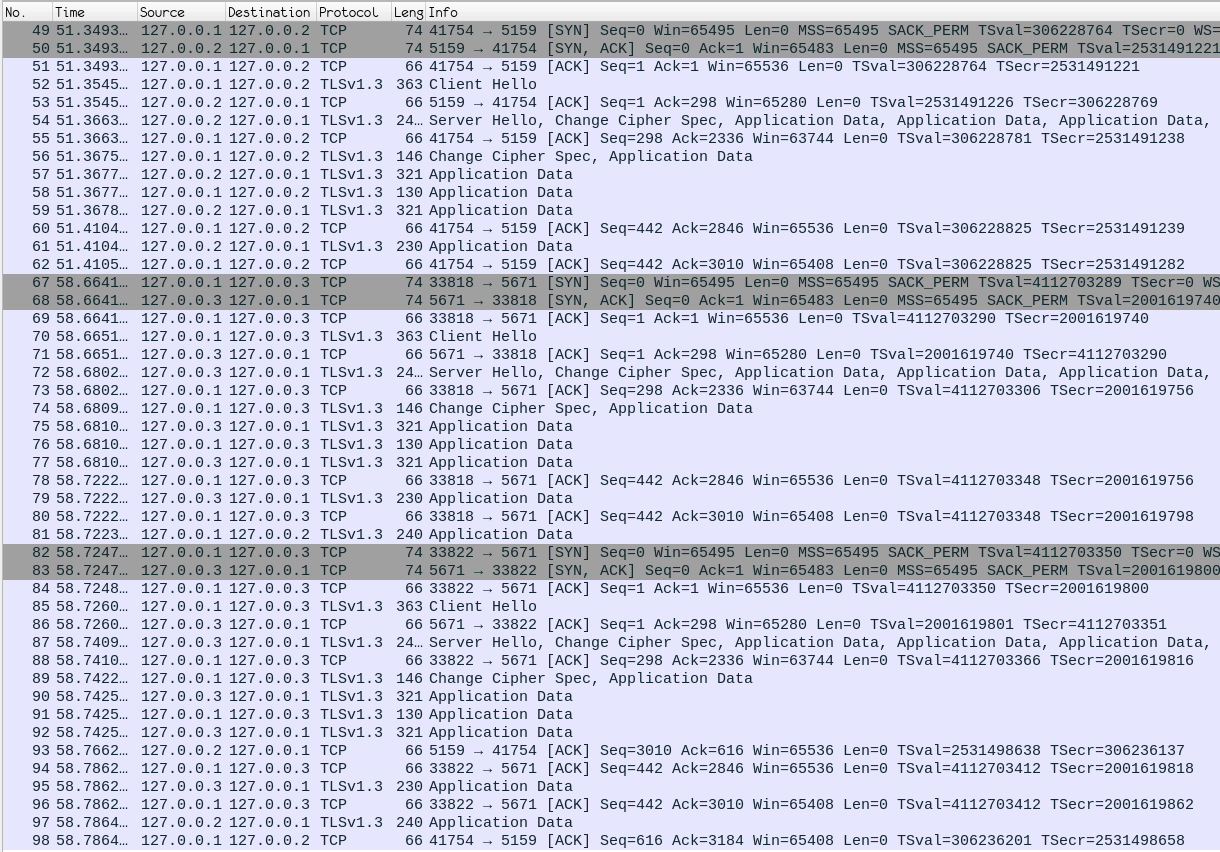
\includegraphics[width=\linewidth]{inc/img/trace-conf-3-tls.png}
  \caption{Сниф wireshark соединения трех участников с использованием TLS}
  \label{img:trace-conf-3-tls}
\end{figure}
